\renewcommand{\typeRubriek}{loep}		

%%%%%%%%%%%%%%%%%%%%%%%%%%%%%
% informatie voor de auteur %
%%%%%%%%%%%%%%%%%%%%%%%%%%%%%
% de soorten titels opmaakmogelijkheden die de auteur kan gebruiken:
% section
% section*, betekent dat er geen nummer bij gezet wordt
% subsection
% tussentitel
% citaat
% opsomming
% nummering
% bronnen
% kader
% stellingkader (genummerd)
% stellingkadertwee (niet genummerd)
% kleurkader
% werktekst



% twee parameters voor nieuwe rubriek: titel en auteur (die mogen ook leeggelaten worden o.a. voor redactioneel)
\startNieuweRubriek{Creatieve instappen in de eerste graad}{Cinder Neyens\\}

\startcontents[mainsections]		      % om opsomming in inhoudstafel enkel tot loep te beperken
\begin{multicols}{2}                      
\inhoudstafelLoep		                  % om inhoudstafel in te voegen



%%%%%%%%%%%%%%%%%%%%%%%%%%%%%%%%%%%%%%%%%%%%%%%%%%%%%%%%%%%%%%%%
%%%%%%%%%%%           START VAN DE TEKST               %%%%%%%%%%
%%%%%%%%%%%%%%%%%%%%%%%%%%%%%%%%%%%%%%%%%%%%%%%%%%%%%%%%%%%%%%%%

\section{Inleiding}
Ik ben Cinder Neyens, studente in de lerarenopleiding Educatieve Bachelor Secundair Onderwijs voor de onderwijsvakken wiskunde en natuurwetenschappen in Howest Brugge. Voor mijn bachelorproef deed ik onderzoek naar het gebruik van creatieve instappen in de wiskundeles in de eerste graad A-stroom. Het onderwerp van deze bachelorproef was een voorstel van mijn lector wiskunde en promotor voor dit onderzoek, Kelly Schedin. Zij pikte het idee om creatieve instappen te verzamelen op in een gesprek met een wiskundeleerkracht tijdens een stageobservatie. In de opleiding tracht zij ons op verschillende manieren duidelijk te maken dat wiskunde geven een hele mooie uitdaging is, waarbij creativiteit en een goede basisvorming centraal staan. Uit mijn onderzoek bleek dat heel wat wiskundeleerkrachten de les graag op een leuke manier willen starten maar hier om verschillende redenen niet toe komen. Het vele voorbereidingswerk en het gebrek aan inspiratie zijn de boosdoeners. Bovendien vinden zij het veel eenvoudiger om een creatieve instap te vinden voor meetkunde dan voor getallenleer. Dit komt omdat meetkunde zeer visueel is en getallenleer abstractere onderwerpen bevat. Ook bleek dat de leerlingen het een grote meerwaarde vinden om de les te starten met een leuke inleiding. Het motiveert hen en wekt hun interesse voor het verdere verloop van de les. 

\begin{center}
wiskundeinstappen.wordpress.com
\end{center}

is de website die ik creërde en waarop voor heel wat wiskundige onderwerpen uit de eerste graad A-stroom een instap terug te vinden is. De website is dynamisch en heeft een dubbele functie. Je kunt de kant en klare instappen enerzijds rechtstreeks toepassen in de klas. Dit vergt weinig voorbereidingswerk, waardoor de drempel om gebruik te maken van een leuke inleiding lager wordt. Anderzijds kan het platform ook dienen als inspiratiedoos, waarbij een instap naar eigen wensen aangepast kan worden. 

Op de website wordt elke instap volgens een vast sjabloon stapsgewijs omschreven. Daarnaast geef ik bij elke instap de tijdsinvestering in de klas, de groepsgrootte, de groeperingsvorm, de hoeveelheid voorbereidend werk, het al dan niet nodig hebben van ICT, het dynamisch aspect en de benodigdheden. Op de overzichtspagina’s kun je in één oogopslag zien aan welke criteria de instappen voldoen en wordt meteen duidelijk welke instappen al dan niet uitvoerbaar zijn met je klas. Niet alle instappen hebben dezelfde rol. Sommige instappen zijn enkel bedoeld om de aandacht op het onderwerp van de les te richten. Andere instappen gaan een stuk verder en zorgen reeds voor de aanbreng van de leerstof.

Tot slot is er nog een pagina “Creëer je eigen instap”. Op deze pagina zijn er blanco en bewerkbare modellen, zoals lege bingo- en dominokaarten, terug te vinden. Je kunt met de blanco modellen zelf een instap creëren voor een onderwerp naar keuze. Daarnaast zijn verschillende werkvormen uitbreidbaar tot andere onderwerpen en graden. Zo kun je bijvoorbeeld de instap “Wie ben ik?” vertalen naar een instap over functies in de tweede graad.

\section{Meetkunde}

\subsection{Wie ben ik?}
De onderstaande instap kan gebruikt worden om de eigenschappen van vierhoeken te herhalen. Deze instap wordt in duo’s gespeeld en vergt weinig voorbereidingswerk. De leerkracht moet enkel de onderstaande kaartjes en plakband voorzien. 

\tussentitel{Stap 1}
Er worden duo’s gevormd. Elk duo heeft acht kaartjes nodig, namelijk een vierkant, rechthoek, parallellogram, gelijkbenige trapezium, ongelijkbenige trapezium, ruit, vlieger en willekeurige vierhoek.

\tussentitel{Stap 2}
De kaartjes worden op de bank gelegd met de blanco kant naar boven gericht. Leerling 1 kiest een kaartje en plakt dit met plakband op het hoofd van leerling 2 zonder dat die ziet wat er op het kaartje staat.
\tussentitel{Stap 3}
Leerling 2 moet ja-neenvragen stellen i.v.m. de zijden, hoeken en diagonalen van de vierhoek om te achterhalen welk kaartje er op zijn of haar hoofd plakt. Mogelijke vragen zijn: 
\begin{opsomming} 
\item Heb ik vier gelijke zijden?
\item Heb ik twee paar evenwijdige zijden?
\item Heb ik vier rechte hoeken?
\item Staan mijn diagonalen loodrecht op elkaar?
\item Zijn mijn diagonalen even lang?
\item Snijden mijn diagonalen elkaar middendoor?
\item Zijn mijn overstaande hoeken even groot?
\end{opsomming}

De benaming van de vierhoek moet zo specifiek mogelijk zijn.

\tussentitel{Stap 4}
Nadat leerling 2 achterhaald heeft welk kaartje op zijn of haar hoofd plakt, wordt er gewisseld. Leerling 2 kiest vervolgens een kaartje en plakt dit op het hoofd van leerling 1.
De duo’s blijven doorgaan totdat alle kaartjes aan bod zijn gekomen. 
\end{multicols}

\begin{figure}[H]
\begin{center}
\includegraphics[width=\linewidth]{img/Linstappen_vierhoeken.png}
\captionof{figure}{De kaartjes van 'Wie ben ik?'}
\end{center}
\end{figure}

 \begin{multicols} {2}
De leerlingen herhalen de verschillende soorten vierhoeken met de bijbehorende eigenschappen op een speelse manier.

\tussentitel{Suggestie}
Maak er een wedstrijdje van en daag de leerlingen uit om te weten te komen welke vierhoek ze zijn in zo weinig mogelijk vragen.

 \subsection{Meten met je lichaam}
 De volgende instap heeft betrekking tot lengtematen en hoeken. Met behulp van hun lichaam gaan de leerlingen allerlei zaken opmeten, zeer beweeglijk dus! Het is zeer functioneel, want de leerlingen hebben hun lichaam altijd bij zich! Deze instap vergt opnieuw weinig voorbereiding. Als leerkracht dien je een lintmeter en enkele opdrachten te voorzien zoals:
 \begin{opsomming} 
\item Meet de omtrek van het klaslokaal;
\item Bereken de oppervlakte van de bank waaraan je zit;
\item Bepaal de omtrek van het bord;
\item Bepaal de oppervlakte van de deur;
\item Meet de lengte van de gang;
\item Bepaal de lengte van een pennenzak.
\end{opsomming}

\tussentitel{Stap 1}
Laat de leerlingen hun persoonlijk meetinstrument voor een meter, decimeter en centimeter op hun lichaam bepalen met een lintmeter. Dit kan verschillen van leerling tot leerling.

\begin{center}
\includegraphics[width=\linewidth]{img/Lmeten_arm.png}
\captionof{figure}{Een persoonlijke meter:
de afstand van de schouder van de ene kant van het lichaam t.e.m. de hand aan de uitgestrekte arm aan de andere kant van het lichaam bedraagt ongeveer 1 m.}
\end{center}
\end{multicols}

\begin{figure}[H]
\begin{center}
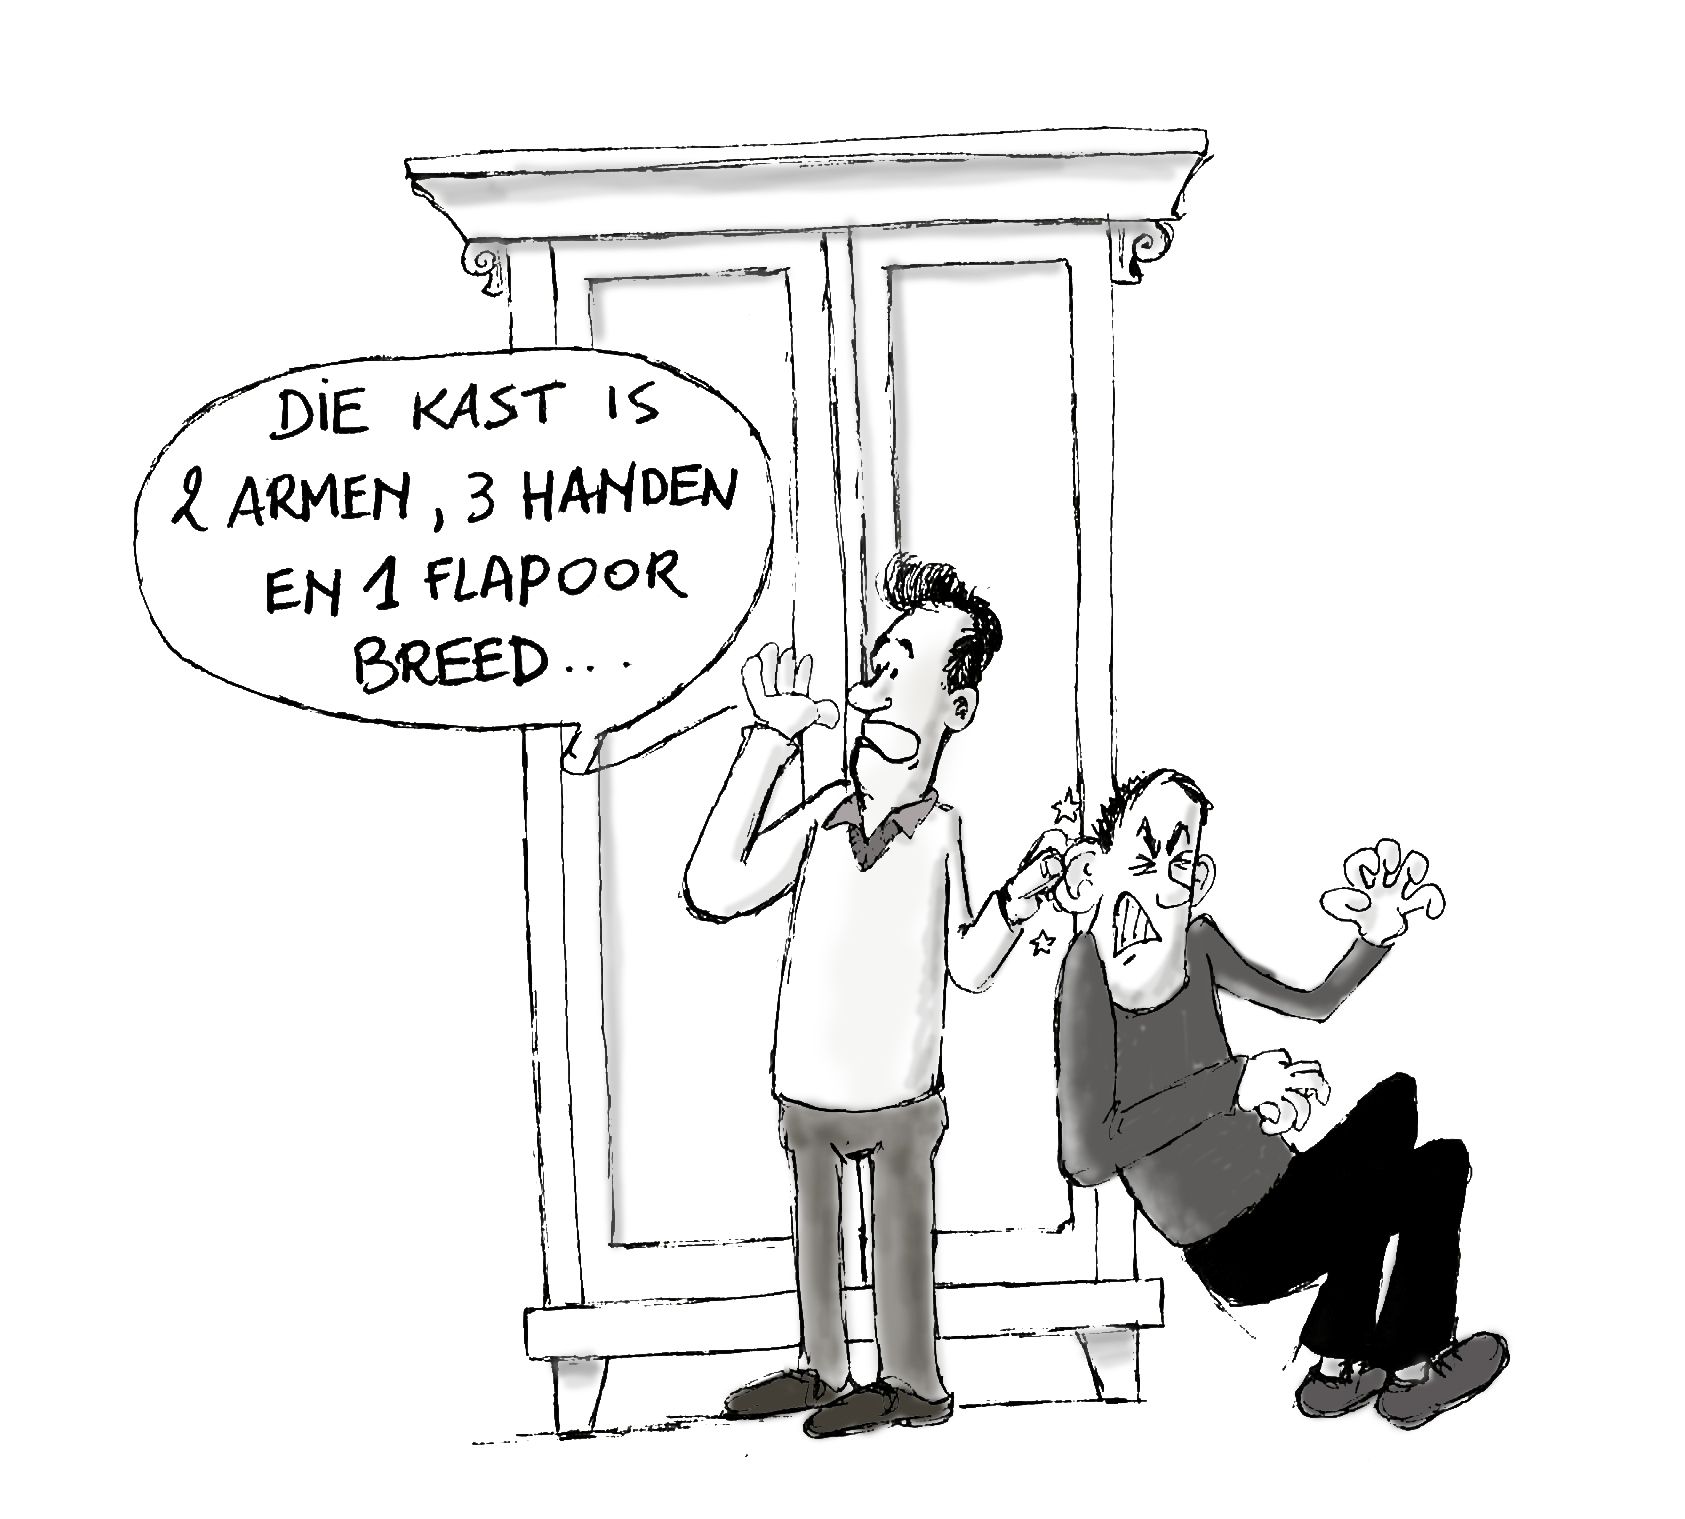
\includegraphics[width=0.75\linewidth]{img/Lkast.jpg}

\end{center}
\end{figure}

\begin{multicols} {2}
 
\begin{center}
\includegraphics[width=\linewidth]{img/Lmeten_ogen.png}
\captionof{figure}{Een persoonlijke decimeter:
de afstand tussen de buitenkanten van de ogen bedraagt ongeveer 1 dm (= 10 cm). 
}
\end{center}

\begin{center}
\includegraphics[width=\linewidth]{img/Lmeten_vinger.png}
\captionof{figure}{Een persoonlijke centimeter:
de dikte van een vinger bedraagt ongeveer 1 cm. Elke leerling bepaalt voor zichzelf welke vinger dit is.}
\end{center} 

\tussentitel{Stap 2}
Als alle leerlingen hun persoonlijke meetinstrumenten bepaald hebben, geeft de leerkracht hen opdrachten. De leerlingen proberen m.b.v. hun lichaam lengtes, omtrekken of oppervlakten te berekenen.

\tussentitel{Suggestie: maak je eigen gradenboog}
Niet alleen om lengtes te meten, maar ook om hoeken te meten kunnen we ons lichaam gebruiken. Je kunt hier opnieuw een opdracht aan koppelen. De leerlingen kunnen een hoek eerst schatten met behulp van hun handen en die daarna opmeten met een meetinstrument.

\begin{center}
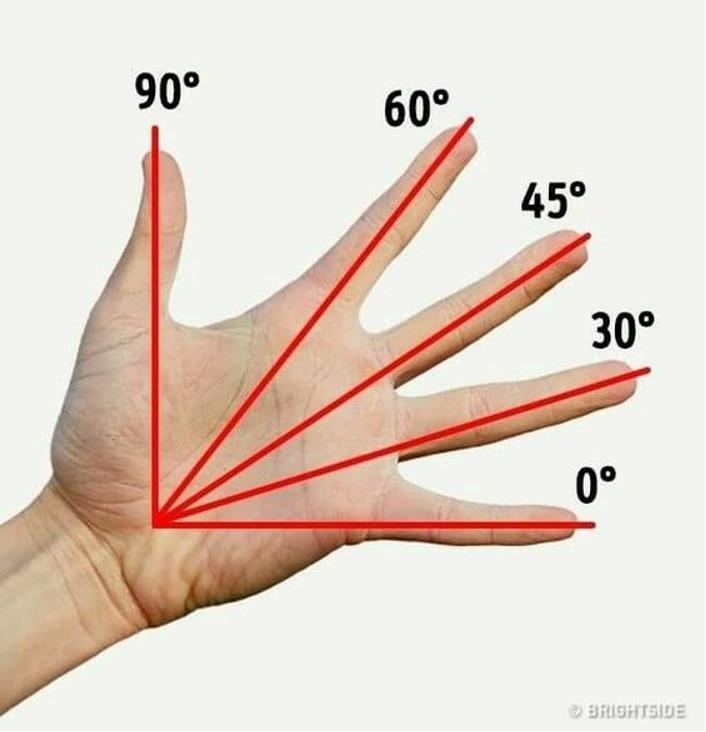
\includegraphics[width=\linewidth]{img/Lmeten_graden.jpg}
\captionof{figure}{Je hand gebruiken als gradenboog}

\end{center} 

\subsection{Jantje verschuift}

De volgende instap is een variatie op het spel “Jantje zegt” als inleiding op een les over verschuivingen. Tijdens dit spel voeren de leerlingen verschuivingen uit, een actieve inleiding op dit leerstofonderdeel.
Deze instap duurt niet lang en zorgt voor beweging, ideaal dus aan het begin van de les. 
\tussentitel{Stap 1}
De leerkracht legt het spel en geeft aan hoelang er gespeeld wordt.
\begin{opsomming}
\item Regel 1: Als de leerkracht “Jantje zegt …” voor een instructie zegt, dan moeten de leerlingen dit wel doen.
\item Regel 2: Als de leerkracht meteen de instructie geeft zonder “Jantje zegt…”, dan moeten de leerlingen dit niet doen.
\end{opsomming}
	
\tussentitel{Stap 2}
Het spel wordt gespeeld. Leerlingen die een instructie uitvoeren, terwijl dit niet de bedoeling was, moeten gaan neerzitten. Enkele mogelijke instructies zijn:
\begin{opsomming}
\item Zet twee stappen naar links.
\item Spring 3 maal naar voor.
\item Slide naar achteren.
\item Slide naar rechts.
\item Loop naar voor en tik de muur.
\item Kruip op handen en voeten 2 stappen naar voor.
\item Ga hurken en zet 1 stap naar achteren.
\item Doe je ogen toe en zet 4 stappen naar rechts.
\item Zet 3 stappen schuin naar linksachter.
\item Draai rond je as.
\end{opsomming}

De laatste instructie staat erbij om duidelijk te maken dat niet alle bewegingen verschuivingen zijn.
\tussentitel{Stap 3}
Blik terug op de verschillende verschuivingen die de leerlingen uitvoerden in de ruimte en koppel dit aan de les.

\tussentitel{Suggestie}
Als er te weinig plaats is, kan een vijftal leerlingen naar voor komen of kan de instap buiten plaatsvinden.
 
\end{multicols}

\begin{figure}[H]
\begin{center}
\includegraphics[width=\linewidth]{img/Lperspectief.png}
\captionof{figure}{Voorbeelden van spelen met perspectief}
\end{center}
\end{figure}

\begin{multicols} {2}
\subsection{Spelen met perspectief}
Dit is een hele uitdagende en korte instap waarbij de leerlingen creatief aan het werk gaan met perspectieven. 

\tussentitel{Stap 1}
Geef de leerling de voorgaande les de opdracht om een foto te maken waarbij ze spelen met perspectieven. Geef hen de voorbeelden uit figuur 6 mee. Deze opdracht mogen ze alleen of samen met een vriend uitvoeren. Daag hen uit om creatief te zijn!

\tussentitel{Stap 2}
Projecteer de foto’s die de leerlingen gemaakt hebben in de klas.
\tussentitel{Stap 3}
Vertel vervolgens dat je in een vlakke afbeelding niet alle informatie uit de driedimensionale ruimte kunt vatten waardoor ze zo’n gekke afbeeldingen konden maken.

In de werkelijkheid is er bijvoorbeeld heel wat afstand tussen de twee personen op de onderstaande afbeelding. De ene staat veraf en lijkt daarom kleiner dan de persoon die dichtbij staat. We nemen dit echter niet waar op deze vlakke afbeelding. Daar heeft de fotograaf precies voor gezorgd.

\begin{center}
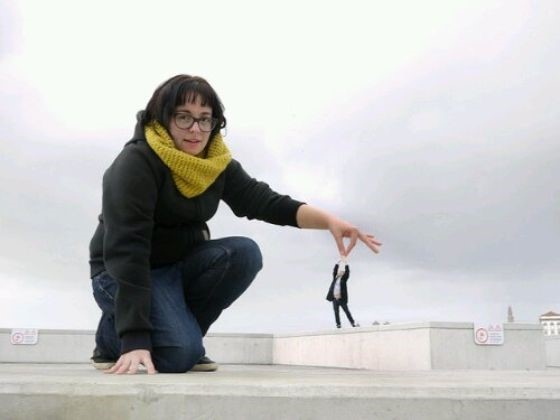
\includegraphics[width=\linewidth]{img/Lperspectief2.jpg}
\captionof{figure}{Wat is de afstand tussen de twee personen op de foto?}
\end{center}

Maar wat als we die ruimte wel in kaart willen brengen op een vlak stuk papier? Dan kunnen we tekenen in perspectief! We verliezen steeds informatie als we van 3D naar 2D gaan. Nu kan de les omtrent perspectieven starten. 

\section{Getallenleer}
\subsection{Kennismakingshoepels}
Verzamelingen worden gebruikt om de verbanden tussen verschillende soorten getallen te beschrijven. Deze instap is een beweeglijke kennismakingsoefening gekoppeld aan bewerkingen met verzamelingen. De leerkracht brengt twee hoepels uit de sportzaal en post-its mee naar de klas.
\tussentitel{Stap 1}
Geef elke leerling een post-it waarop ze hun naam noteren en leg vooraan in de klas één hoepel zoals op de onderstaande afbeelding.

\begin{center}
\includegraphics[width=\linewidth]{img/Lverzamelingen1.png}
\captionof{figure}{Een hoepel als voorstelling van een verzameling}

\end{center} 

\tussentitel{Stap 2}
Stel enkele kennismakingsvragen (je kiest zelf hoeveel).
Enkele voorbeelden:
\begin{opsomming}
\item Wie komt met de fiets naar school?
\item Wie heeft een broer?
\item Wie draagt lenzen?
\item Wie heeft TikTok?
\item Wie zit in een sportclub?
\item Wie speelt een muziekinstrument?
\item …
\end{opsomming}

De leerlingen die aan de vraag voldoen, plaatsen hun post-it binnenin de hoepel en de anderen hun post-it buiten de hoepel.

De plaats binnen de hoepel noemen we een verzameling. In dit geval is het de verzameling van de leerlingen die aan de vraag voldoen. De plaats binnen én buiten de hoepel noemen we de universele verzameling. In dit geval alle namen van de leerlingen uit de klas.

Na het stellen van enkele vragen kan het begrip “element” geïntroduceerd worden. Bijvoorbeeld tijdens het stellen van de vraag “Wie draagt een bril?” ligt de post-it van Jan in de cirkel. Dit wil zeggen dat Jan een element is van deze verzameling.
\tussentitel{Stap 3}
Neem er een tweede hoepel bij en plaats die zoals op de onderstaande afbeelding.

\begin{center}
\includegraphics[width=0.9\linewidth]{img/Lverzamelingen2.png}
\captionof{figure}{Twee verzamelingen}

\end{center} 

Elke hoepel stelt een verzameling voor. Stel opnieuw enkele vragen, maar verwijs in je formulering naar het begrip verzameling.
\begin{opsomming}
\item Ik wil links de verzameling van alle leerlingen met bruine ogen en rechts de verzameling van alle leerlingen die een bril dragen.
\item Ik wil links de verzameling van alle leerlingen die dansen en rechts de verzameling van alle leerlingen die met de bus naar school komen. 
\item …
\end{opsomming}

Er zal ongetwijfeld verwarring ontstaan. De leerlingen zullen zich afvragen wat ze moeten doen als ze tot beide verzamelingen behoren. Laat hen wat discussiëren en probeer tot slot tot het onderstaande resultaat te komen. 
\begin{center}
\includegraphics[width=0.9\linewidth]{img/Lverzamelingen3.png}
\captionof{figure}{Een betere voorstelling van twee verzamelingen}

\end{center} 

\end{multicols}

\begin{figure}[H]
\begin{center}
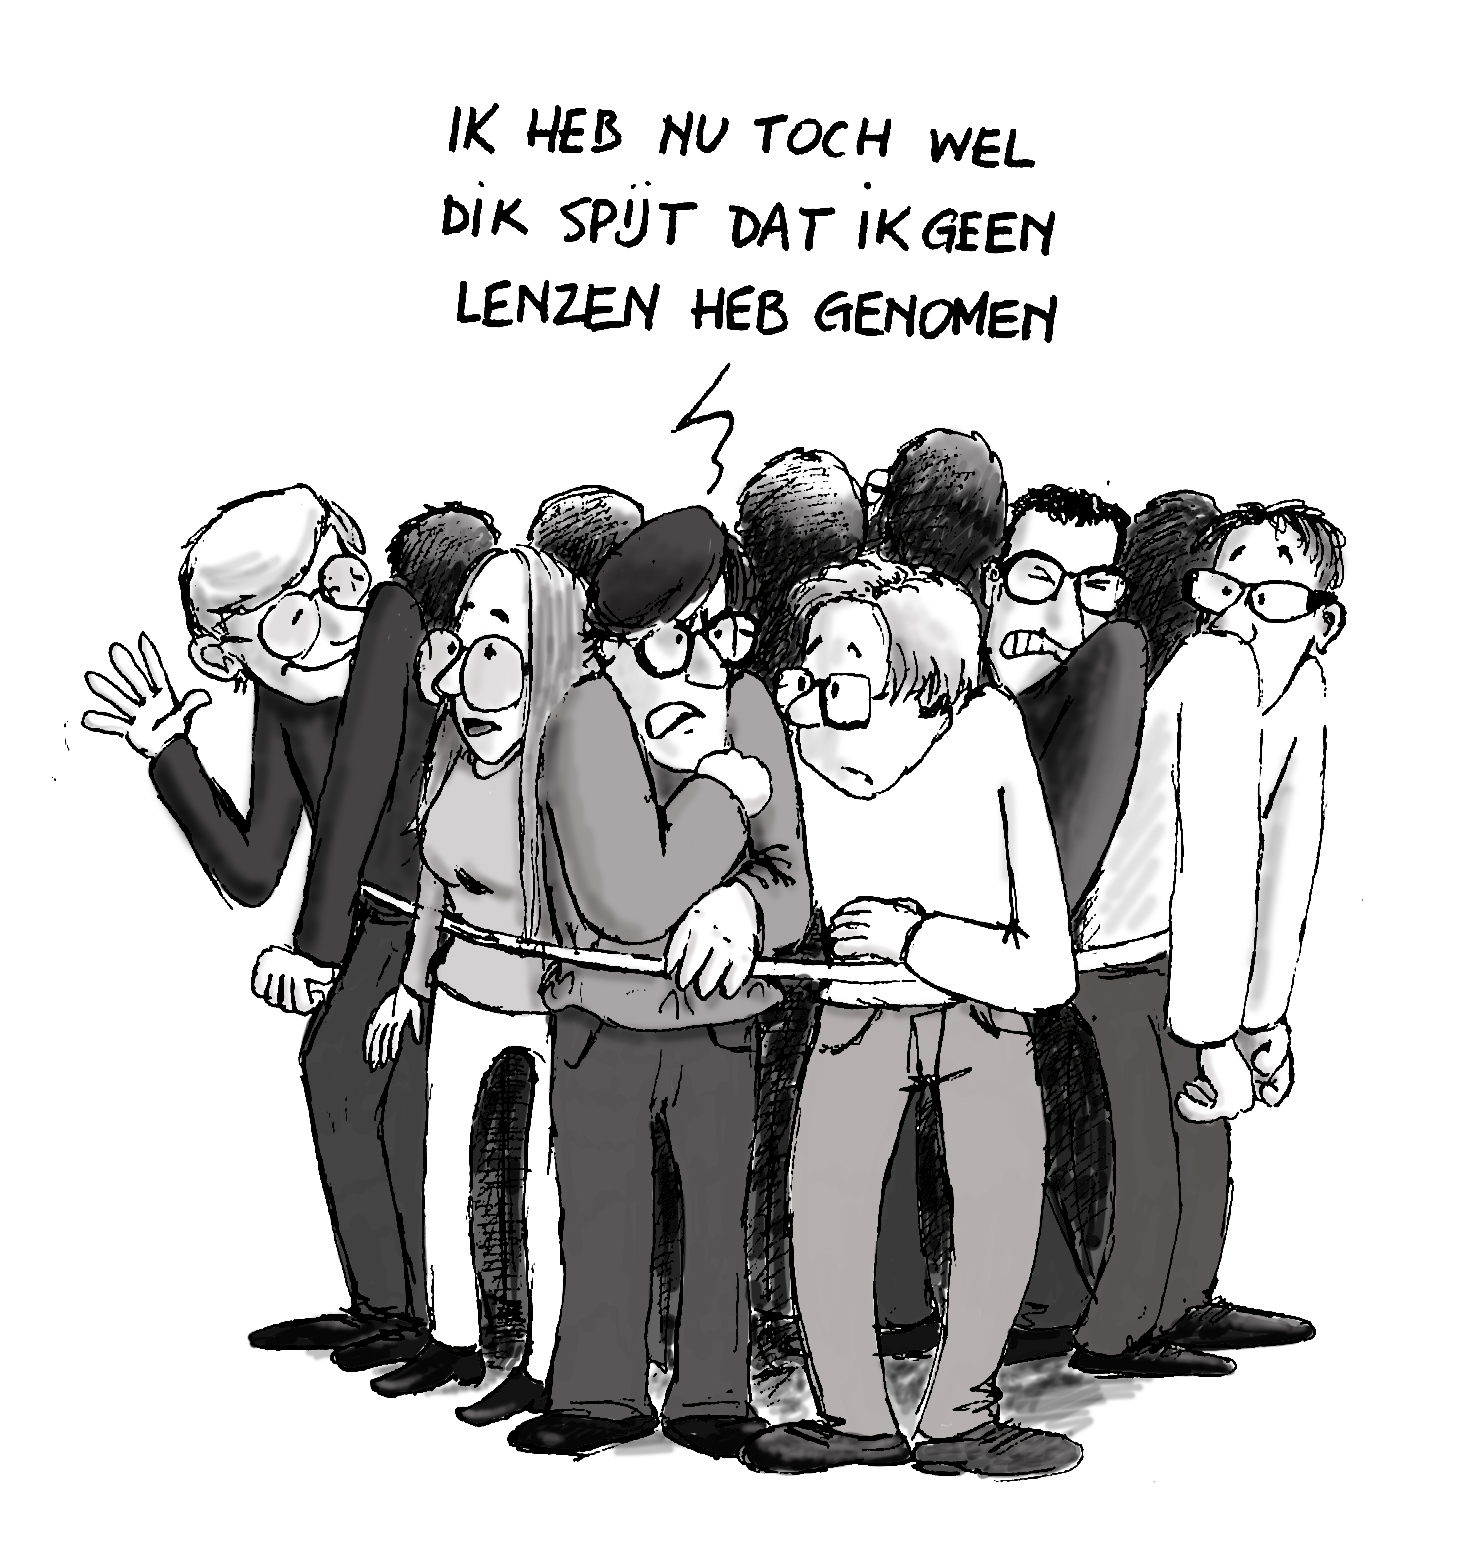
\includegraphics[width=0.7\linewidth]{img/Lhoepel.jpg}

\end{center}
\end{figure}

\begin{multicols} {2}
 
Introduceer vervolgens het begrip “doorsnede”. De doorsnede is de ruimte waar de twee cirkels elkaar overlappen. 

\tussentitel{Stap 4}
Tot slot ga je met een laatste voorbeeldje alle begrippen herhalen. 

Bijvoorbeeld: aan de linkerkant bevindt zich de verzameling van alle leerlingen die een bril dragen en rechts bevindt zich de verzameling van alle leerlingen die fan zijn van LikeMe.

\begin{center}
\includegraphics[width=\linewidth]{img/Lverzamelingen4.png}
\captionof{figure}{Twee verzamelingen met enkele elementen erin}

\end{center} 

Vervolgens stel je enkele vragen om de begrippen aan te kaarten.
\begin{opsomming}
\item Geef mij een element uit de doorsnede van de verzamelingen bril en LikeMe. Dit wil zeggen een leerling die zowel een bril draagt als fan is van LikeMe.

\emph{Antwoord: Ann of Veerle}
\item Geef mij een element uit de unie van de verzamelingen bril en LikeMe. Dit wil zeggen een leerling die een bril draagt of fan is van LikeMe.  

\emph{Antwoord: Iedereen behalve Kim en Tibo}
\item Geef mij een element uit het verschil van de verzamelingen bril en LikeMe. Dit wil zeggen een leerling die een bril draagt, maar geen fan is van LikeMe.

\emph{Antwoord: Sara, Tim, Luca en Sam}
\end{opsomming}


Indien nodig kun je nog voorbeelden verzinnen.


\subsection{Facebookpost}
Op Facebook circuleert de rekensom uit figuur 12. 


\begin{center}
\includegraphics[width=\linewidth]{img/LFacebook.png}
\captionof{figure}{Een populaire rekensom op Facebook}

\end{center} 

We gebruiken die als instap voor de les rond de volgorde van de bewerkingen. Het is een klassikale instap waarbij gebruik kan worden gemaakt van een digitale tool. Opnieuw komt er niet veel voorbereidingswerk bij kijken. De leerkracht moet enkel de bovenstaande bewerking aan de leerlingen geven.

\tussentitel{Stap 1}
Vraag de leerlingen om de bewerking uit te voeren. De leerlingen schrijven hun antwoord op een stukje papier. Digitale suggestie: je kunt de app Mentimeter gebruiken om de leerlingen met hun smartphone laten antwoorden. Deze app zet een digitale poll meteen om in een statistisch diagram.

\tussentitel{Stap 2}
De leerkracht gaat rond en haalt alle antwoorden op. De antwoorden zijn anoniem. 

\tussentitel{Stap 3}
De antwoorden worden overlopen en geturfd. 
Er komt verwarring op bij de leerlingen. Het lijkt zo’n simpele opgave. Het zijn getallen onder 10, super gemakkelijk! En toch merken de leerlingen bij hun klasgenoten heel wat verschillende antwoorden op …
\tussentitel{Stap 4}
Toon de onderstaande grafiek aan de leerlingen.


\begin{center}
\includegraphics[width=\linewidth]{img/LFacebook2.png}
\captionof{figure}{Overzicht van de antwoorden op Facebook}

\end{center} 

Op de grafiek zien de leerlingen de antwoorden van Facebookgebruikers staan. Ook daar zijn heel wat verschillende antwoorden, net zoals in de klas!

\tussentitel{Stap 5}
De leerkracht geeft aan dat het juiste antwoord 8 is.
De leerkracht kan hier inspelen op de verbazing en hen prikkelen om te weten hoe ze het juiste antwoord kunnen verkrijgen. Het antwoord hierop is dat ze de volgorde van bewerkingen moeten respecteren. Het feit dat de vraag van Facebook komt, werkt motiverend.

\tussentitel{Suggestie}
Je kunt hier nog dieper op ingaan en de leerlingen uitdagen met een foutenanalyse. Vraag hen welke fouten er gemaakt werden bij de andere uitkomsten. Zo rekenden de mensen die “1” antwoordden bijvoorbeeld van links naar rechts zonder rekening te houden met de volgorde van de bewerkingen.


\subsection{Snoepzakjes vullen}

Aan de hand van het vullen van snoepzakjes maken de leerlingen kennis met de grootste gemene deler. Voor deze korte instap heb je enkele zakjes of bekertjes nodig en snoepjes.

\tussentitel{Stap 1}
Stel de klas de volgende vraag: “Ik heb snoepjes voor mij liggen, namelijk 42 M\&M’s, 36 beertjes en 24 colaatjes. Ik wil hiermee zoveel mogelijk gelijke snoepzakjes maken en ik wil natuurlijk alle snoepjes uitdelen. Hoeveel gelijke snoepzakjes kan ik maken?”

\begin{center}
\includegraphics[width=\linewidth]{img/Lsnoepjes1.png}
\captionof{figure}{Snoepjes om te verdelen over gelijke snoepzakjes}

\end{center}

\tussentitel{Stap 2}
Laat de leerlingen zoeken naar het antwoord. 

Wanneer enkele leerlingen denken het antwoord gevonden te hebben, vraag hen dan hoe ze te werk zijn gegaan. Indien je merkt dat de leerlingen niet starten met berekeningen, probeer hen dan een tip te geven. Laat de leerlingen met één soort snoepjes beginnen en laat de voorwaarde om zoveel mogelijk zakjes te vullen vallen. Vraag hoeveel zakjes je kunt maken. Op deze manier worden de leerlingen op het spoor van delers gezet. De stap naar gemeenschappelijke delers is dan snel gemaakt. Het getal 1 is een deler van de drie getallen. Hoeveel zakjes heb ik dan? Maar ik wil graag zoveel mogelijk gelijke snoepzakjes maken …

\tussentitel{Stap 3}
Vervolgens kun je samen met de klas alle delers van de drie getallen zoeken en kijken welke delers ze gemeenschappelijk hebben, om er tot slot de grootste deler die ze gemeenschappelijk hebben uit te halen. (Antwoord: 6)

\begin{center}
\includegraphics[width=\linewidth]{img/Lsnoepjes2.png}
\captionof{figure}{De delers van 24, 36 en 42}

\end{center} 

\tussentitel{Stap 4}
Maak de snoepzakjes en controleer of het klopt wat de leerlingen berekend hebben. 

In elk snoepzakje zitten 4 colaatjes, 6 beertjes en 7 M\&M’s.

\begin{center}
\includegraphics[width=\linewidth]{img/Lsnoepjes3.png}
\captionof{figure}{De oplossing: 6 gelijke snoepzakjes!}

\end{center} 

\tussentitel{Stap 5}
Haal tot slot aan dat je zo’n vraagstuk kunt oplossen door te zoeken naar de grootste gemene deler. De g.g.d. van 24, 36 en 42 is namelijk 6.
Hierna kunnen de snoepjes uiteraard opgegeten worden, mmm.

\section{Algebra en analyse}
\subsection{Coördinatenslag}

Deze instap bereidt de leerlingen voor op een les rond de coördinaten van punten. De leerlingen werken in duo’s en de leraar dient enkel zeeslagkaarten voor elke leerling af te drukken. 

\begin{center}
\includegraphics[width=0.9\linewidth]{img/Lzeeslag1.png}
\captionof{figure}{Een zeeslagkaart}

\end{center} 

\tussentitel{Stap1}
Elke leerling krijgt een zeeslagkaart met twee roosters en elke leerling haalt een groene en rode kleur boven.

\tussentitel{Stap 2}
De leerlingen vormen duo's, zitten over elkaar en plaatsen een map tussen hen in.
\tussentitel{Stap 3}
Elke leerling plaatst op het onderste deel van zijn of haar blad een aantal boten. Een boot van 5 vakjes, 4 vakjes, 3 vakjes en 2 vakjes. Ze doen dit door de vakjes in te kleuren met een potlood. De boten mogen niet tegen elkaar liggen, ook niet met hoekjes!
\tussentitel{Stap 4}
Leerling 1 stelt een vraag aan leerling 2. Bijvoorbeeld: “Staat er een boot op vakje 1,2?”
Als het antwoord ja is, dan zet leerling 1 een groen kruisje op het bovenste deel van zijn of haar blad. Vervolgens zet leerling 2 een groen kruisje op het onderste deel van zijn of haar blad.
Als het antwoord neen is, dan wordt hetzelfde gedaan als hierboven, maar met rode kruisjes.

\tussentitel{Stap 5}
Nu is het de beurt aan leerling 2 om een vraag te stellen aan leerling 1.

Let op: de leerlingen zullen snel merken dat ze nood hebben aan afspraken. Vermelden we eerst het getal op de horizontale of dat op de verticale as? De leerkracht maakt duidelijk dat we eerst de horizontale as en daarna de verticale as geven. Op die manier oefenen de leerlingen het correct aflezen van coördinaten, want daarbij wordt ook steeds eerst de $x$-coördinaat en vervolgens de $y$-coördinaat afgelezen.

\tussentitel{Stap 6}
De leerlingen blijven doorspelen totdat iemand alle boten van de tegenstander gevonden heeft of totdat de leerkracht aangeeft dat het tijd is om te stoppen.

Door deze instap gaan de leerlingen de noodzaak inzien om consequent eerst de $x$-coördinaat en vervolgens de $y$-coördinaat af te lezen. De overgang naar de les over coördinaten zal vlot verlopen, aangezien ze de link zullen kunnen leggen met het spel zeeslag dat ze zopas gespeeld hebben. 
\end{multicols}

\begin{figure}[H]
\begin{center}
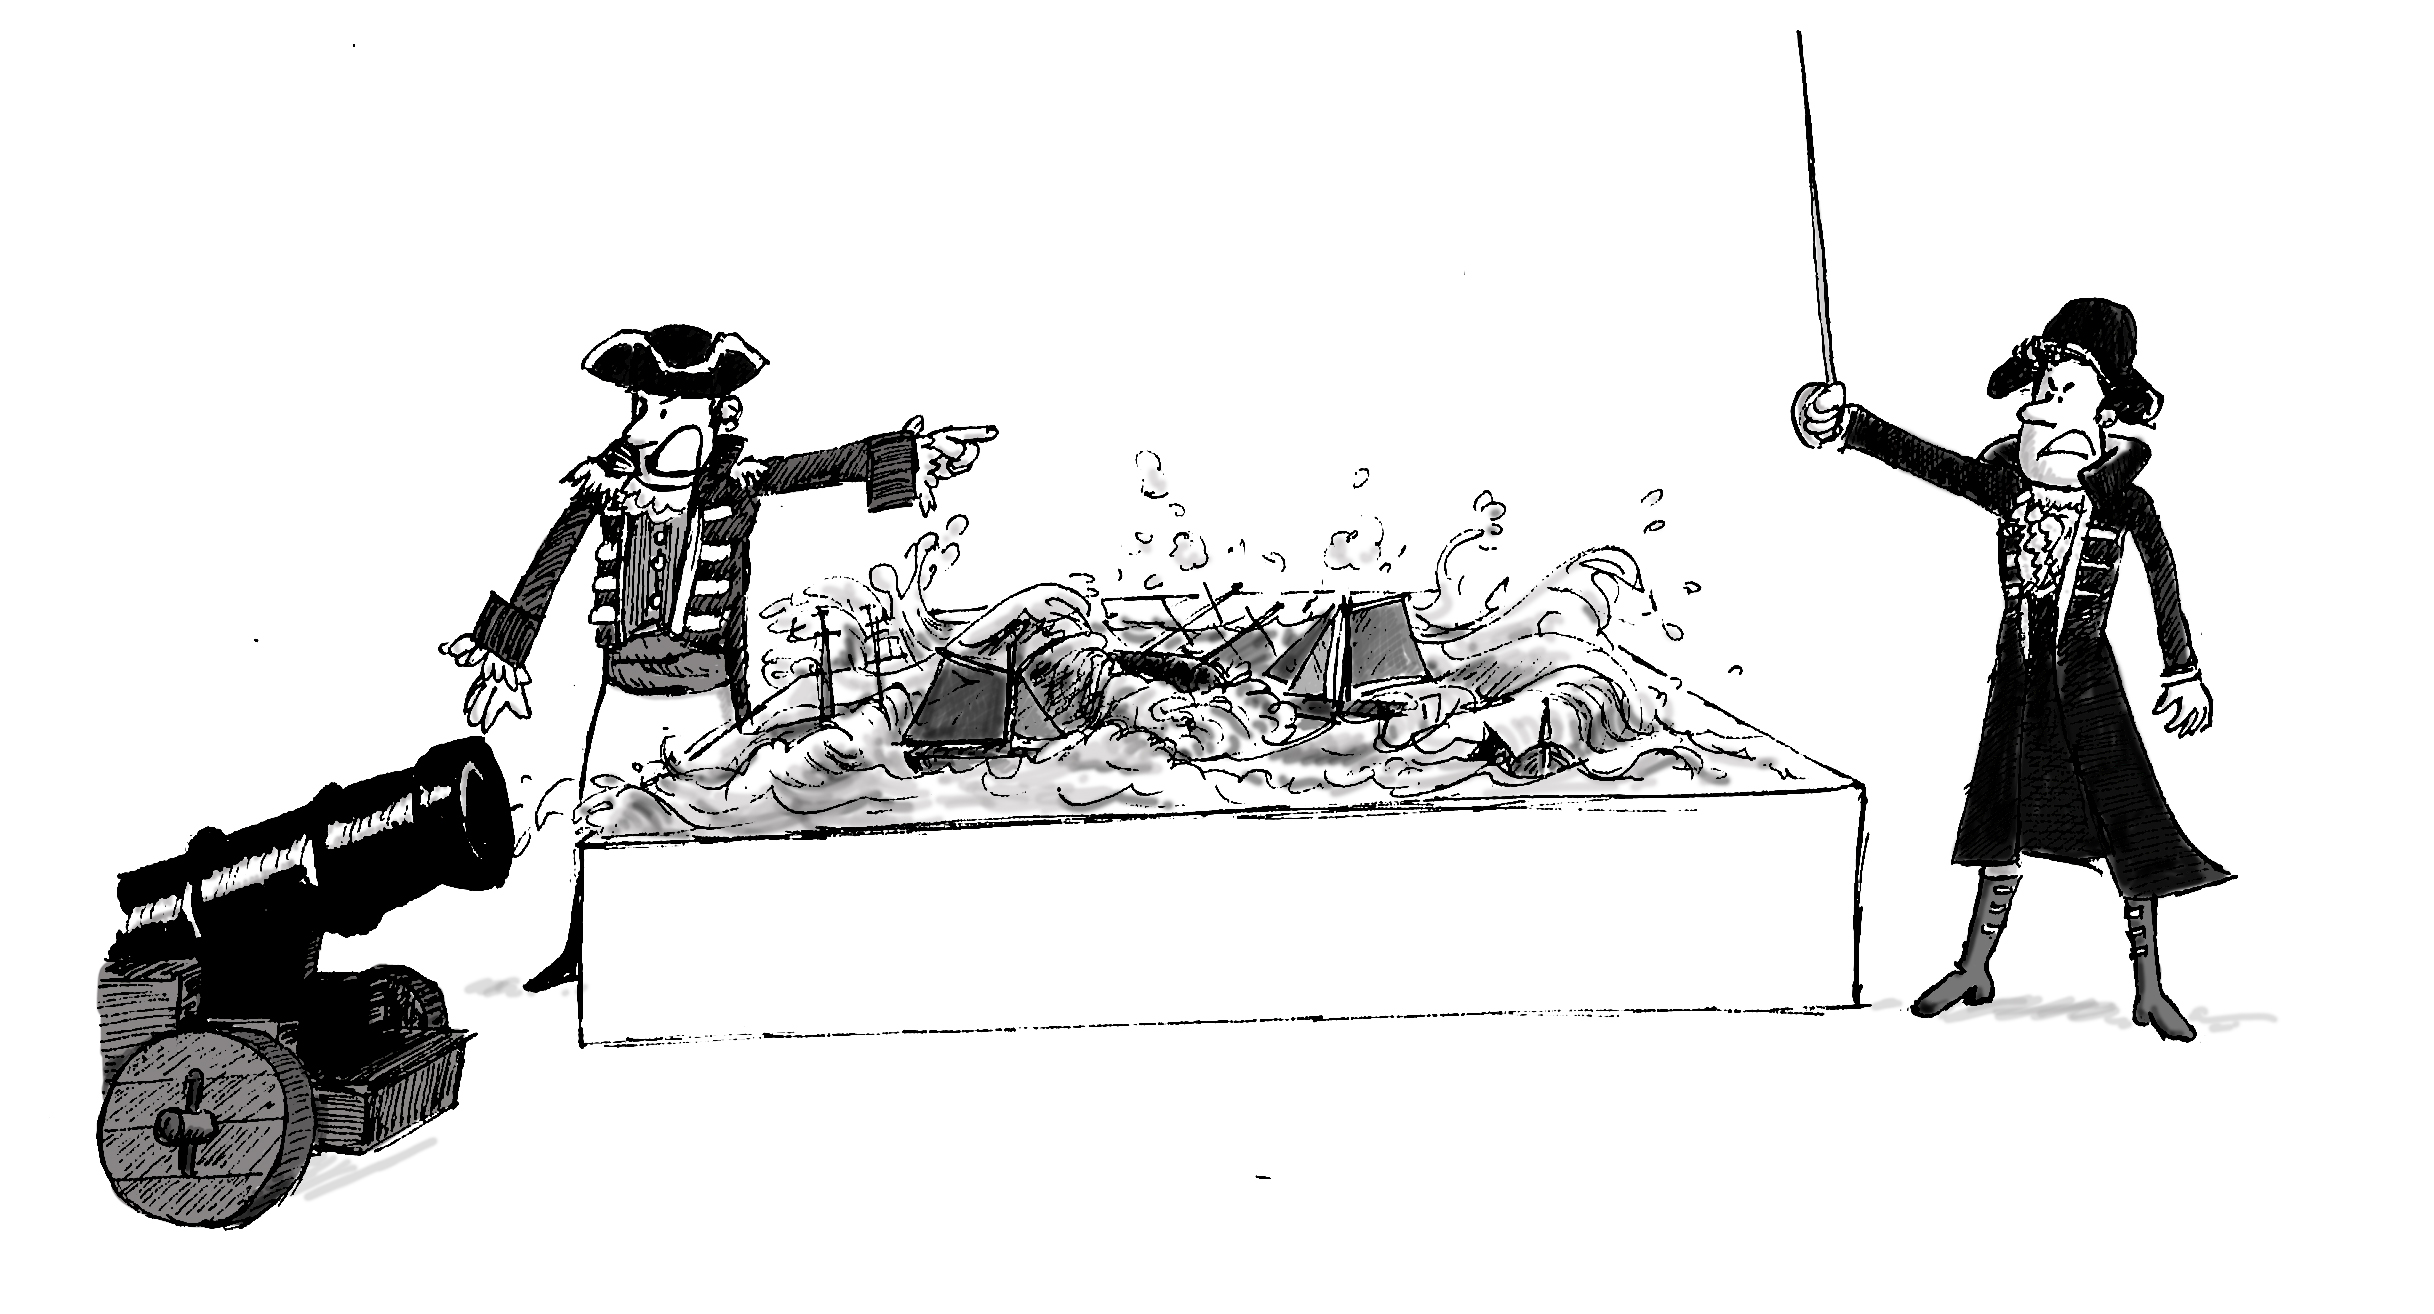
\includegraphics[width=0.9\linewidth]{img/Lzeeslag.jpg}

\end{center}
\end{figure}

\begin{multicols} {2}
Ze zullen zich minder snel vergissen tussen de volgorde van de $x$- en $y$-as tijdens het aflezen van de coördinaten. 

Opgelet: Tijdens dit spel stellen de vakjes de coördinaten voor. Tijdens je les moet je de leerlingen erop wijzen dat de coördinaten geen vakjes meer voorstellen, maar roosterpunten.

\subsection{Merkwaardige productenrace}
Deze instap is een inleiding op een les over het product van toegevoegde tweetermen. Het is een wedstrijdje snelrekenen waarbij de leerkracht het opneemt tegen de leerlingen. Voor deze instap is geen materiaal nodig en er wordt veel bewogen.

\tussentitel{Stap 1}
Iedereen staat op eenzelfde afstand van het bord, bv. 2 meter. De leerkracht noteert een bewerking op het bord bv. “$78 \cdot 82$”. Indien de leerlingen de leerkracht ervan verdenken vals te spelen en de bewerkingen op voorhand uitgerekend te hebben, kun je een leerling het eerste getal laten bepalen (bv. 93). De leerkracht kiest hierna meteen de tweede factor van het product, namelijk “87”. En dan start de race.

\tussentitel{Stap 2}
Zowel de leerkracht als de leerlingen proberen de bewerking zo snel mogelijk uit te voeren. De leerlingen mogen hun rekenmachine gebruiken en de leerkracht rekent uit het hoofd. Wie het antwoord heeft, loopt ze zo snel mogelijk naar het bord en schrijft het op.

\tussentitel{Stap 3}
De leerkracht zal in de meeste gevallen het antwoord als eerste op het bord kunnen schrijven omdat hij of zij gebruik maakt van het merkwaardig product en de bewerking als volgt uitvoert: 

$78 \cdot 82 = (80 - 2)(80 + 2) = 80^2 - 2^2 = 6400 - 4 = 6396$

De leerlingen zullen verontwaardigd zijn en zich afvragen hoe het mogelijk is dat de leerkracht voor hen het antwoord weet, terwijl zij hun rekenmachine mogen gebruiken. Op die manier worden ze getriggerd en gemotiveerd om dit ook te kunnen. Ze zullen gemotiveerd worden om merkwaardige producten te leren.
\tussentitel{Suggestie}
Indien het steeds dezelfde leerling is die het antwoord als eerste op het bord kan schrijven, kun je die leerling een ‘handicap’ geven, zoals 2 meter extra naar achteren beginnen of 5 seconden later starten.

\subsection{TikToktwins}
Bij deze instap maken de leerlingen kennis met het kwadraat van een tweeterm a.d.h.v. een filmpje. Het is een korte instap die weinig voorbereiding vergt en inspeelt op de leefwereld van de leerlingen. Leerlingen van de eerste graad zijn namelijk verzot op de app TikTok.

\tussentitel{Stap 1}
Toon de video (https://youtu.be/2WKzoUlWU-8) in de klas.

\begin{center}
\includegraphics[width=\linewidth]{img/Ltiktok.png}
\captionof{figure}{De TikToktwins}
\end{center}


\tussentitel{Stap 2}
De video geeft aan dat $(a + b)^2 = a^2 + 2ab + b^2$. De leerlingen zullen verbaasd zijn en zich afvragen of dit effectief zo is. Ze zullen dit willen onderzoeken. Je kunt dat laten onderzoeken door getallen in te vullen (iedereen kiest andere getallen). Daarna kun je op zoek gaan naar een verklaring aan de hand van een algemene bewerking of een meetkundige verklaring. 

Op deze manier kan de les over het kwadraat van een tweeterm ingeleid worden. De leerlingen zullen getriggerd zijn om dit te onderzoeken. Het feit dat het filmpje een TikTok is, zal de leerlingen aanspreken, aangezien dit het interessegebied van de leerlingen van de eerste graad is.

\tussentitel{Suggestie}
Laat de leerlingen een TikTokvideo maken waarin ze het kwadraat van een tweeterm uitleggen. Dit neemt uiteraard meer tijd in beslag. Het is geen instap meer, maar wel een verwerkingsopdracht.

\subsection{Chocolademousse}
Tijdens deze instap maken de leerlingen kennis met verhoudingen aan de hand van een recept om chocolademousse te maken. Het vergt weinig voorbereidingswerk. Het enige wat je als leerkracht moet doen, is enkele recepten afdrukken en het aan je leerlingen geven. Tijdens deze instap werken de leerlingen in groepjes.
\tussentitel{Stap 1}
Verdeel de klas in 4 groepen.

\tussentitel{Stap 2}
Geef elke groep een recept. 
De leerkracht vertelt dat hij chocolademousse wil maken, maar enkel een recept voor 4 personen vindt. Hij weet niet welke hoeveelheden hij moet gebruiken als hij dit enkel wil maken voor hemzelf en zijn partner (2 personen) of voor zijn gezin (5 personen) of voor zijn familie (11 personen) of voor de volledige klas (20 personen). 
Elke groep krijgt een ander aantal personen (zie figuren 19 en 20) en probeert de correcte hoeveelheden te achterhalen.

\begin{center}
\includegraphics[width=\linewidth]{img/Lchocolademousse1.png}
\captionof{figure}{Het recept voor 4 en 5 personen}
\includegraphics[width=\linewidth]{img/Lchocolademousse2.png}
\captionof{figure}{Het recept voor 4 en 20 personen}
\end{center}

\tussentitel{Stap 3}
Als iedereen klaar is, legt elke groep aan de rest van de klas uit hoe zij aan hun antwoorden komen.
De kans is groot dat ze voor 5 en 11 personen de regel van drie toepassen. Hopelijk doen ze dat niet voor 2 en 20 personen. Hierbij is het eenvoudiger om de ingrediënten te halveren of te vervijfvoudigen. 
\tussentitel{Stap 4}
Na de uitleg van elke groep vertelt de leerkracht dat de ingrediënten uit een recept voor $n$ personen evenredig zijn met de ingrediënten uit het recept voor 4 personen. Dit wil zeggen dat de verhoudingen bij elk recept dezelfde blijven. 
Met deze instap is het onderwerp evenredigheden ingeleid.

\section{Statistiek}
\subsection{Het grote M\&M-onderzoek}
De onderstaande instap introduceert de begrippen gemiddelde, mediaan, modus en variatiebreedte. Het is een instap die langer duurt dan de andere instappen die hier reeds besproken werden. Hiervoor zijn een zak M\&M’s en bekertjes nodig. 

\tussentitel{Stap 1}
Teken het schema uit tabel 1 op het bord. Verdeel de klas in duo’s en verdeel de zak M\&M’s over de plastic bekertjes. Doe dit door in elke beker een gelijk aantal M\&M’s te gieten.

\tussentitel{Stap 2}
Elk duo sorteert hun M\&M’s per kleur, zoals je kunt zien bij het middelste duo op de foto uit figuur \ref{tafelmm}.

\begin{center}
\includegraphics[width=\linewidth]{img/LMenM.png}
\captionof{figure}{Het tellen van de M\&M's}
\label{tafelmm}
\end{center}

\tussentitel{Stap 3}
Elk duo telt de rode, groene, bruine, gele, blauwe en oranje M\&M’s die in hun potje zitten. Ze wandelen naar het bord en vullen hun gegevens op de juiste plaats in het bordschema in.
\tussentitel{Stap 4}
Nadat de volledige tabel is aangevuld, vult de leerkracht het schema verder aan (zie tabel \ref{tab: tabel2}).

\end{multicols}
\begin{table}[H]
 \centering
 \begin{tabular}{|l||r|r|r|r|r|r|}\hline
  Groepje&	Rood&	Bruin& Geel& Groen& Blauw& Oranje\\\hline
  Duo 1&	& & &  &  & \\\hline
  Duo 2&	& & &  &  & \\\hline
  Duo 3&	& & &  &  & \\\hline
   ...&	& & &  &  & \\\hline
  \end{tabular}
  \caption{De tabel die de duo's moeten aanvullen}
  \label{tab: tabel1}
 \end{table}

\begin{multicols}{2}

\end{multicols}
\begin{table}[H]
 \centering
 \begin{tabular}{|l||r|r|r|r|r|r|}\hline
  &	Rood&	Bruin&	Geel& Groen& Blauw& Oranje\\\hline
Gemiddelde&	& & &  &  & \\\hline
Mediaan&	& & &  &  & \\\hline
Modus&	& & &  &  & \\\hline
Variatiebreedte&	& & &  &  & \\\hline
  \end{tabular}
  \caption{De tabel waarin de centrummaten en variatiebreedte ingevuld kunnen worden}
  \label{tab: tabel2}
 \end{table}

\begin{multicols}{2}


\tussentitel{Stap 5}
Met de volledige klas samen ga je na wat het gemiddeld aantal rode M\&M’s in een potje is, indien de zak M\&M’s willekeurig is uitgegoten over de potjes. Ook de mediaan, modus en variatiebreedte van de rode M\&M’s onderzoek je samen met de klas. Vervolgens wordt dit door de leerlingen herhaald voor de andere 5 kleuren M\&M’s.

Op die manier maken de leerlingen op een leuke en experimentele manier kennis met de basisbegrippen van de statistiek, namelijk het gemiddelde, de mediaan, de modus en de variatiebreedte.
De ingevulde tabel kan er dan uitzien zoals in tabel 3.

Je kunt dan stilstaan bij de betekenis van de verschillende centrummaten in deze context. Het gemiddelde geeft aan hoeveel rode M\&M’s je zou hebben als iedereen er evenveel had. Je moet alles optellen en delen door het aantal duo's:
$$(8+4+2+8+6+5+5+4+5) : 9 = 5,2.$$
Het gemiddelde is dus 5,2 M\&M’s.

De mediaan is het middelste getal van de geordende rij die het aantal rode M\&M’s voorstelt. Het middelste getal van de rij

$$2, 4, 4, 5, 5, 5, 6, 8, 8$$

is 5. De mediaan is dus 5 rode M\&M’s.

De modus is het aantal rode M\&M’s dat het meest voorkomt? Het aantal 2 komt éénmaal voor, 4 en 8 tweemaal en 5 driemaal. Bijgevolg komt 5 het meeste voor en is 5 de modus voor de rode M\&M’s.

De variatiebreedte ten slotte is het verschil tussen het hoogste en het laagste aantal rode M\&M’s. Dit is $8-2 =  6$ en bijgevolg is de variatiebreedte 6.

Tot slot kunnen de M\&M’s natuurlijk ook lekker opgegeten worden!

\subsection{Dominodiagram}
De laatste instap van dit artikel is een instap waarin de leerlingen kennis maken met verschillende soorten diagrammen. De leerkracht voorziet voor elk duo een setje dominokaartjes.

\end{multicols}
\begin{table}[H]
 \centering
 \begin{tabular}{|l||r|r|r|r|r|r|}\hline
  Groepje&	Rood&	Bruin&	Geel& Groen& Blauw& Oranje\\\hline
Duo 1&	8& 6& 6&  5&  7& 7\\\hline
Duo 2&	4& 6& 5&  8&  4& 5\\\hline
Duo 3&	2& 7& 9&  1&  9& 6\\\hline
Duo 4&	8& 3& 4&  10&  2& 5\\\hline
Duo 5&	6& 6& 6&  6&  7& 8\\\hline
Duo 6&	5& 4& 5&  8&  5& 8\\\hline
Duo 7&	5& 4& 8&  5&  7& 6\\\hline
Duo 8&	4& 5& 7&  8&  4& 6\\\hline
Duo 9&	5& 3& 5&  4&  9& 8\\\hline
&	& & &  &  & \\\hline
Gemiddelde&	5,2& 4,9& 6,1&  6,1&  6& 6,5\\\hline
Mediaan&	5& 5& 6&  6&  7& 6\\\hline
Modus&	5& 6& 5&  8&  7& 6 en 8\\\hline
Variatiebreedte&	6& 4& 5&  9&  7& 3\\\hline
  \end{tabular}
  \caption{Een voorbeeld van een volledig ingevulde tabel}
  \label{tab: tabel3}
 \end{table}

\begin{center}
\includegraphics[width=0.85\linewidth]{img/Ldomino1.png}

\includegraphics[width=0.85\linewidth]{img/Ldomino2.png}
\end{center}
\begin{multicols}{2}

\tussentitel{Stap 1}
De klas wordt verdeeld in duo’s. Elk duo krijgt een setje dominokaarten.
\tussentitel{Stap 2}
Elk duo probeert hun domino te vervolledigen. Op de dominokaartjes staan heel wat verschillende diagrammen (ringdiagram, spreidingsdiagram, staafdiagram, cirkeldiagram, watervaldiagram, trechterdiagram, strookdiagram, lijndiagram, vlakdiagram en treemap). De leerlingen moeten de diagrammen die dezelfde gegevens weergeven aan elkaar koppelen en de slinger vervolledigen.
\tussentitel{Stap 3}
Om de instap af te sluiten vertelt de leerkracht dat de leerlingen a.d.h.v. het dominospel gemerkt hebben dat er heel wat verschillende soorten diagrammen zijn. Er bestaan heel wat verschillende manieren om gegevens te visualiseren, maar de leerlingen zullen zich in het lesvervolg focussen op de staaf-, lijn-, spreidings- en cirkeldiagram.
Het eindresultaat vind je op de vorige pagina terug. Deze afbeelding kun je eventueel projecteren als alle duo’s klaar zijn. Op die manier hoef je niet bij elk duo langs te gaan, maar kunnen de leerlingen zichzelf controleren.

Zoals eerder vermeld is er ook een blanco model van de dominokaartjes terug te vinden op de pagina “Creëer je eigen instap” op mijn website. Zo kun je ook voor andere onderwerpen de les starten met een dominospel.


Ik heb hier een tiental van mijn ontworpen creatieve instappen besproken, maar op mijn site kun je er nog veel meer terugvinden. 

Veel plezier!

\end{multicols}

\stopcontents[mainsections]			        % altijd laten staan, opsomming in inhoudstafel enkel tot loep beperken
